\chapter{Specifikacija programske potpore}
		
	\section{Funkcionalni zahtjevi}
			
			\noindent \textbf{Dionici:}
			
			\begin{packed_enum}
				
				\item Vlasnik (naručitelj)
				\item Članovi organizacije
				
				\begin{packed_enum}
					\item Zaposlenik
					\item Revizor
					\item Računovođa
					\item Direktor
				\end{packed_enum}
				
				\item Administrator
				\item Razvojni tim
				
			\end{packed_enum}
			
			\noindent \textbf{Aktori i njihovi funkcionalni zahtjevi:}
			
			
			\begin{packed_enum}
				
				\item  \underbar{Neregistrirani/neprijavljeni korisnik (inicijator) može:}
				\begin{packed_enum}
					
					\item se prijaviti u sustav pomoću kredencijala (e-mail adresa i lozinka) koje je dobio od superriornije osobe 
					
				\end{packed_enum}
			
				\item  \underbar{Zaposlenik (inicijator) može:}
				\begin{packed_enum}
					
					\item prijaviti se u sustav
					\item pregledati svoje osobne podatke (ime, prezime, nadređeni revizor)
					\item skenirati dokumente koje se spremaju u njegovu internu bazu
					\item potvrditi dokumente koje je prethodno skenirao
					\item poslati revizirane dokumente od njegove strane na dodatan pregled
					\item vidjeti svoju internu bazu prethodno skeniranih dokumenata
					
				\end{packed_enum}
				
				\item  \underbar{Revizor (inicijator) može:}
				\begin{packed_enum}
					
					\item prijaviti se u sustav
					\item pregledati svoje osobne podatke (ime, prezime, popis podređenih zaposlenika)
					\item dobiti obavijesti o skeniranim dokumentima od strane podređenog zaposlenika
					\item skenirati dokumente koje se spremaju u njegovu internu bazu
					\item revizirati primljene dokumente
					\item proslijediti određenom računovođi dokument skeniran i potvrđen od strane podređenog zaposlenika
					
				\end{packed_enum}
				
				\item  \underbar{Računovođa (inicijator) može:}
				\begin{packed_enum}
					
					\item prijaviti se u sustav
					\item pregledati svoje osobne podatke (ime, prezime, vrstu dokumenta za koju je zaslužan)
					\item pregledati dokumente spremne za arhiviranje
					\item arhivirati dokumente
					\item pregledati povijest dokumenata koje je arhivirao u svojoj internoj bazi
					\item prosljediti dokumente direktoru na potpis prije dokumentiranja 
					
				\end{packed_enum}
				
				\item  \underbar{Direktor (inicijator) može:}
				\begin{packed_enum}
					
					\item prijaviti se u sustav
					\item pregledati svoje osobne podatke (ime, prezime, ime tvrtke za koju je zaslužan)
					\item primati obavijesti o zatraženim potpisima o računovođi
					\item pregledati popis svih korisnika aplikacije
					\item pregledati statistike zaposlenika (broj skeniranih dokumenata,
					prosjek skeniranih dokumenata svih zaposlenika te ostale statistike)
					\item promjeniti uloge i ostale podatke o svim ostalim korisnicima unutar tvrtke 
					\item brisati račune otpuštenih zaposlenika tvrtke te stvarati 
					\item pregledati sve dokumente i njihovu povijest(tko ih je skenirao, 
					revizirao i koji računovođa je bio zaslužan za njihovo arhiviranje)
					\item objaviti određeni dokument na društvenim mrežama
					
				\end{packed_enum}
				
				\item  \underbar{Administrator (inicijator) može:}
				\begin{packed_enum}
					
					\item prijaviti se u sustav
					\item dodavati različite tvrtke i njihove direktore
					\item pregledati osobne podatke svih korisnika aplikacije
					\item upozoravati direktora na kršenje uvijete poslovanja aplikacije
					\item brisati korisnika koji krše uvijete poslovanja aplikacije
					
				\end{packed_enum}
				
				\item  \underbar{Baza podataka (sudionik) može:}
				\begin{packed_enum}
					
					\item pohraniti podatke o svim korisnicima aplikacije
					\item pohraniti sve podatke o tvrtkama te arhivitra sve dokumente određene tvrtke
					
				\end{packed_enum}
				
				
			\end{packed_enum}
			
			\eject 
			
			
				
			\subsection{Obrasci uporabe}
				
				\textbf{\textit{dio 1. revizije}}
				
				\subsubsection{Opis obrazaca uporabe}
					\textit{Funkcionalne zahtjeve razraditi u obliku obrazaca uporabe. Svaki obrazac je potrebno razraditi prema donjem predlošku. Ukoliko u nekom koraku može doći do odstupanja, potrebno je to odstupanje opisati i po mogućnosti ponuditi rješenje kojim bi se tijek obrasca vratio na osnovni tijek.}\\
					

					\noindent \underbar{\textbf{UC$<$broj obrasca$>$ -$<$ime obrasca$>$}}
					\begin{packed_item}
	
						\item \textbf{Glavni sudionik: }$<$sudionik$>$
						\item  \textbf{Cilj:} $<$cilj$>$
						\item  \textbf{Sudionici:} $<$sudionici$>$
						\item  \textbf{Preduvjet:} $<$preduvjet$>$
						\item  \textbf{Opis osnovnog tijeka:}
						
						\item[] \begin{packed_enum}
	
							\item $<$opis korak jedan$>$
							\item $<$opis korak dva$>$
							\item $<$opis korak tri$>$
							\item $<$opis korak četiri$>$
							\item $<$opis korak pet$>$
						\end{packed_enum}
						
						\item  \textbf{Opis mogućih odstupanja:}
						
						\item[] \begin{packed_item}
	
							\item[2.a] $<$opis mogućeg scenarija odstupanja u koraku 2$>$
							\item[] \begin{packed_enum}
								
								\item $<$opis rješenja mogućeg scenarija korak 1$>$
								\item $<$opis rješenja mogućeg scenarija korak 2$>$
								
							\end{packed_enum}
							\item[2.b] $<$opis mogućeg scenarija odstupanja u koraku 2$>$
							\item[3.a] $<$opis mogućeg scenarija odstupanja  u koraku 3$>$
							
						\end{packed_item}
					\end{packed_item}
				
					
				\subsubsection{Dijagrami obrazaca uporabe}
					
					\textit{Prikazati odnos aktora i obrazaca uporabe odgovarajućim UML dijagramom. Nije nužno nacrtati sve na jednom dijagramu. Modelirati po razinama apstrakcije i skupovima srodnih funkcionalnosti.}
				\eject		
				
			\subsection{Sekvencijski dijagrami}
				
				\textbf{\textit{Obrazac uporabe UC2 - Prijava u sustav}}\\
				
				\textit{Korisnik unosi svoje osobne podatke. Sustav provjerava u bazi podataka jesu li uneseni podaci ispravni. Ako jesu, korisnik se prijavi u sustav. No ako uneseni podaci ne odgovaraju niti jednom registriranom korisniku u bazi, sustav korisniku šalje obavijest da su osobni podaci neispravni i daje mu priliku za ponovnu prijavu.}
				\begin{figure}[H]
					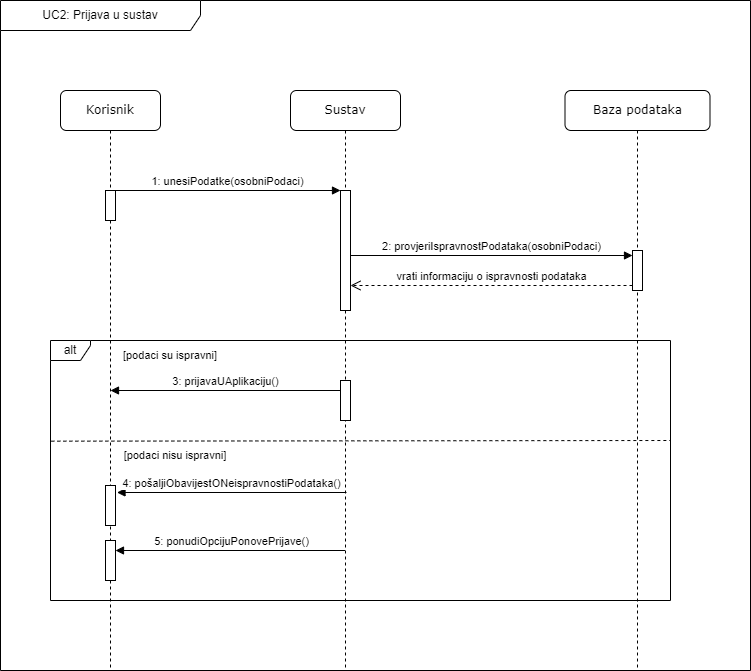
\includegraphics[width=\textwidth]{slike/sekvencijski_dijagram_UC2.PNG} %veličina u odnosu na širinu linije
					\caption{Slika broj: Sekvencijski dijagram za UC2}
					\label{fig:UC2} %label mora biti drugaciji za svaku sliku
				\end{figure}
				\clearpage

				\textbf{\textit{Obrazac uporabe UC9 - Pregled skeniranih dokumenata}}\\
				
				\textit{Korisnik odabire pregled popisa svih dokumenata koje je skenirao. Sustav pretraži u bazi njegove skenirane dokumente i vraća ih korisniku na uvid.}
				\begin{figure}[H]
					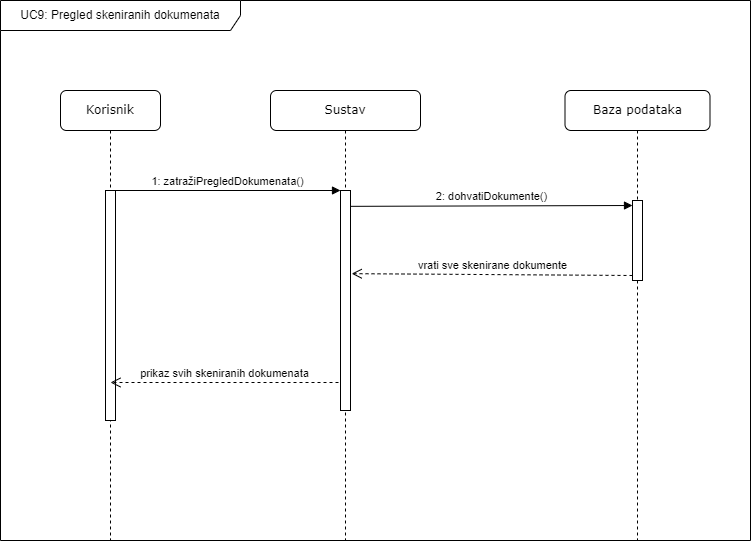
\includegraphics[width=\textwidth]{slike/sekvencijski_dijagram_UC9.PNG} %veličina u odnosu na širinu linije
					\caption{Slika broj: Sekvencijski dijagram za UC9}
					\label{fig:UC9} %label mora biti drugaciji za svaku sliku
				\end{figure}
				\clearpage

				\textbf{\textit{Obrazac uporabe UC21 - Digitalizacija dokumenta}}\\
				
				\textit{Korisnik šalje sliku  u sustav koji zatim tu sliiku učitava i pregledava je li na slici dokument. Ako je, onda na njega primjenjuje OCR te novonastali dokument sprema u bazu podataka. Ako na slici nije očitan dokument, sustav korisniku šalje obavijst da učitana slika ne sadrži dokument te mu daje opciju da priloži novu sliku.}
				\begin{figure}[H]
					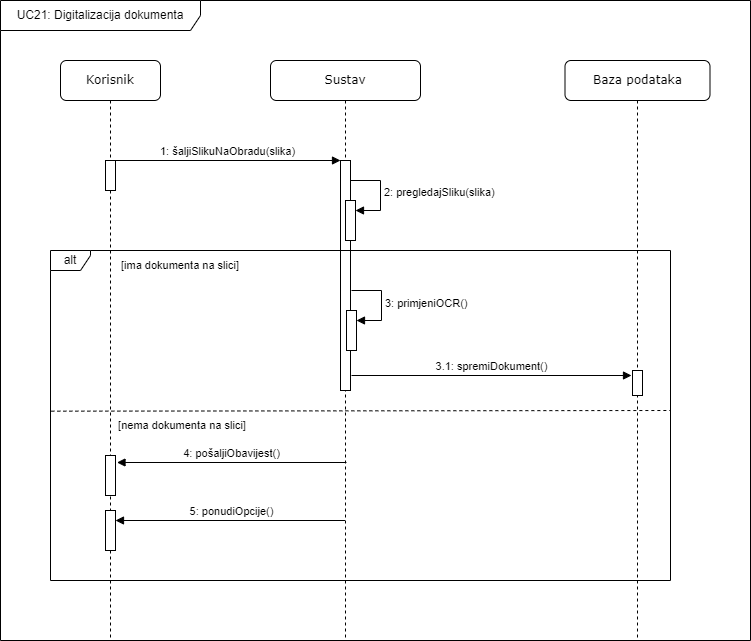
\includegraphics[width=\textwidth]{slike/sekvencijski_dijagram_UC21.PNG} %veličina u odnosu na širinu linije
					\caption{Slika broj: Sekvencijski dijagram za UC21}
					\label{fig:UC21} %label mora biti drugaciji za svaku sliku
				\end{figure}		
				\clearpage

				\eject
	
		\section{Ostali zahtjevi}
		
			\textbf{\textit{dio 1. revizije}}\\
		 
			 \textit{Nefunkcionalni zahtjevi i zahtjevi domene primjene dopunjuju funkcionalne zahtjeve. Oni opisuju \textbf{kako se sustav treba ponašati} i koja \textbf{ograničenja} treba poštivati (performanse, korisničko iskustvo, pouzdanost, standardi kvalitete, sigurnost...). Primjeri takvih zahtjeva u Vašem projektu mogu biti: podržani jezici korisničkog sučelja, vrijeme odziva, najveći mogući podržani broj korisnika, podržane web/mobilne platforme, razina zaštite (protokoli komunikacije, kriptiranje...)... Svaki takav zahtjev potrebno je navesti u jednoj ili dvije rečenice.}
			 
			 
			 
	